The premise of the I-probit model is having regression functions capture the dependence of the covariates on a latent, continuous scale using I-priors, and then transforming these regression functions onto a probability scale.
Therefore, as with the normal I-prior model, an estimate of the posterior regression function with optimised hyperparameters is sought.
A schematic diagram depicting the I-probit model is shown in \cref{fig:iprobitdag}.

\begin{figure}[hbt]
  \centering
  \begin{tikzpicture}[scale=1, transform shape]
    \tikzstyle{main}=[circle, minimum size=10mm, thick, draw=black!80, node distance=16mm]
    \tikzstyle{connect}=[-latex, thick]
    \tikzstyle{box}=[rectangle, draw=black!100]
%      \node[main, draw=black!0] (blank) [xshift=-0.55cm] {};  % pushes image to right slightly
      \node[main, fill=black!10] (x) [] {$x_i$};
      \node[main,double,double distance=0.6mm] (f) [right=of x,yshift=-1.7cm] {$f_{ij}$};
      \node[main] (eta) [below=of x,yshift=-0.7cm] {$\eta$};        
      \node[main] (w) [above=of f,yshift=0.3cm] {$w_{ij}$};  
      \node[main] (ystar) [right=of f,yshift=1.7cm] {$y_{ij}^*$};
      \node[main,double,double distance=0.6mm] (pij) [right=of ystar] {$p_{ij}$};      
      \node[main, fill = black!10] (y) [right=of pij] {$y_{i}$};      
      \node[main] (alpha) [below=of ystar,yshift=-0.75cm] {$\alpha_j$};  
      \node[main, fill=black!10] (Psi) [above=of ystar,yshift=0.4cm] {$\bPsi$};
      \path (alpha) edge [connect] (ystar)
            (eta) edge [connect] (f)
            (x) edge [connect] node [above] {$h$} (f)
    		(f) edge [connect] (ystar)
    		(ystar) edge [connect] node [above] {$g^{-1}$}  (pij)
            (pij) edge [connect] (y)
            (Psi) edge [connect] (w)
            (Psi) edge [connect] (ystar)
    		(w) edge [connect] (f);
      \node[rectangle, draw=black!100, fit={($(x.north west) + (-0.3,0.3cm)$) ($(y.north east) + (0.3,0cm)$) ($(f.south west) + (0,-0.3cm)$) ($(w.north west) + (0,0.3cm)$)}] {}; 
      \node[draw=none] () [below=of y,xshift=-0.3cm,yshift=-0.4cm] {$i=1,\dots,n$};
      \node[rectangle, draw=black!100, fit={($(alpha.south east) + (0,-0.25cm)$) ($(pij.north east) + (0.3,0cm)$) ($(w.north west) + (-0.3,0.58cm)$)  }] {}; 
      \node[draw=none] () [right=of alpha,xshift=-0.4cm,yshift=-0.48cm] {$j=1,\dots,m$};      
    \end{tikzpicture}
    \caption{A directed acyclic graph (DAG) of the I-probit model. Observed or fixed nodes are shaded, while double-lined nodes represents calculable quantities.}
    \label{fig:iprobitdag}
\end{figure}

\index{I-probit!log-likelihood}
The log likelihood function for $\theta$ using all $n$ observations $\{(y_1,x_1),\dots,(y_n,x_n)\}$ is obtained by performing the following integration:
\begin{align}\label{eq:iprobitlik}
  L(\theta|\by) 
  &= \log \iint p(\by|\by^*,\theta) p(\by^*|\bw,\theta) p(\bw|\theta) \dint \by^* \dint \bw.
\end{align}
Here, $p(\bw|\theta)$ is the pdf of $\MN_{n,m}(\bzero,\bI_n,\bPsi)$, $p(\by^*|\bw,\theta)$ is the pdf of $\MN_{n,m}(\bone_n\balpha^\top + \bH_\eta\bw,\bI_n,\bPsi^{-1})$, and $p(\by|\by^*,\theta) = \prod_{i=1}^n \prod_{j=1}^m \big[y_{ij}^* 
    = \max \by^*_{i\bigcdot}\big]^{[y_i = j]}$, with $0^0 := 1$.
Note that, given the corresponding latent propensities $\by^*_{i\bigcdot} = (y_{i1}^*,\dots,y_{im}^*)^\top$, the distribution $y_i|\by^*_{i\bigcdot}$ is tantamount to a degenerate categorical distribution: with knowledge of which latent propensities is largest, the outcome of the categorical response becomes a certainty.

The integral appearing in \cref{eq:iprobitlik} is of order $2nm$, and so presents a massive computational challenge for classical numerical integration methods.
This can be reduced by either integrating out the random effects $\bw$ or the latent propensities $\by^*$ separately.
Continuing on \cref{eq:iprobitlik} gets us to either
\begin{align}
  L(\theta) 
  &= \log \int p(\by|\by^*,\theta) p(\by^*|\theta) \dint \by^* \nonumber \\
  &= \log \int \bigg\{ \prod_{i=1}^n \prod_{j=1}^m \big[y_{ij}^* 
  = \max \by^*_{i\bigcdot}\big]^{[y_i = j]} \bigg\} \,
  \phi(\by^*|\bone_n\balpha^\top, \bPsi \otimes \bH_\eta^2 + \bPsi^{-1} \otimes \bI_n) \dint \by^* \nonumber \\
  &= \log 
  \int_{\bigcap_{i=1}^n  \{ y_{iy_i}^* > y_{ik}^* | \forall k \neq y_i \}}
  \phi(\by^*|\bone_n\balpha^\top, \bPsi \otimes \bH_\eta^2 + \bPsi^{-1} \otimes \bI_n) \dint \by^*, 
  \label{eq:intractablelikelihood1}
\end{align}
by recognising that $\int p(\by^*|\bw,\theta) p(\bw|\theta) \dint \bw$ has a closed-form expression since it is an integral involving two Gaussian densities, or 
\begin{align}
  L(\theta) 
  &= \log \int p(\by | \bw, \theta) \, p(\bw|\theta) \dint \bw \nonumber \\
  &= \log \int \prod_{i=1}^n \Bigg\{ \prod_{j=1}^m \Big( g_j^{-1} \big(  
  \myoverbrace{\balpha + \bw^\top \bh_\eta(x_i)}{\hidewidth \bmu(x_i) \hidewidth}
  \,|\, \bPsi \big) \Big)^{[y_i=j]} \, \phi(\bw_{i \bigcdot}|\bzero,\bPsi) \dint \bw_{i \bigcdot} \Bigg\}, 
  \label{eq:intractablelikelihood2}
\end{align}
where we have denoted the class probabilities $p_{ij}$ from \cref{eq:pij} using the function $g_j^{-1}(\cdot|\bPsi):\bbR^m \to [0,1]$.
Unfortunately, neither of these two simplifications are particularly helpful.
In \cref{eq:intractablelikelihood1}, the integral represents the probability  of a $mn$-dimensional normal variate which is not straightforward to calculate, because its covariance matrix is dense.
In \cref{eq:intractablelikelihood2}, the integral has no apparent closed-form.
The unavailability of an efficient, reliable way of calculating the log-likelihood hampers hope of obtaining parameter estimates via direct likelihood maximisation methods.

Furthermore, the posterior density of the regression function $\bff = \bH_\eta \bw$, which requires the posterior density of $\bw$ obtained via $p(\bw|\by) \propto p(\by|\bw)p(\bw)$, has normalising constant equal to  $L(\theta)$, which is intractable.
The challenge of estimation is then to first overcome this intractability by means of a suitable approximation of the marginalising integral.
We present three possible avenues to achieve this aim, namely the Laplace approximation, a variational EM algorithm, and Markov chain Monte Carlo (MCMC) methods.

\subsection{Laplace approximation}
\index{Laplace's method}

The focus here is to obtain the posterior density $p(\bw|\by) \propto p(\by|\bw)p(\bw) =: e^{R(\bw)}$ which has normalising constant equal to the marginal density of $\by$, $p(\by) = \int e^{R(\bw)} \dint \bw$, as per \cref{eq:intractablelikelihood2}.
Note that the dependence of the pdfs on $\theta$ is implicit, but is dropped for clarity.
Laplace's method \citep[Sec. 4.1.1]{kass1995bayes} entails expanding a Taylor series for $R$ about its posterior mode $\hat\bw = \argmax_\bw p(\by|\bw)p(\bw)$, which gives the relationship
\begin{align*}
  R(\bw) 
  &= R(\hat\bw) + 
  \cancelto{0}{(\bw - \hat\bw)^\top \nabla R(\hat\bw)} 
  - \half (\bw - \hat\bw)^\top \bOmega (\bw - \hat\bw) + \cdots \\
  &\approx R(\hat\bw) + 
  - \half (\bw - \hat\bw)^\top \bOmega (\bw - \hat\bw),
\end{align*}
because, assuming that $R$ has a unique maximum, $\nabla R$ evaluated at its mode is zero.
This is recognised as the logarithm of an unnormalised Gaussian density, implying $\bw|\by \sim \N_n(\hat\bw,\bOmega^{-1})$.
Here, $\bOmega = -\nabla^2 R(\bw)|_{\bw=\hat\bw}$ is the negative Hessian of $Q$ evaluated at the posterior mode, and is typically obtained as a byproduct of the maximisation routine of $R$ using gradient or quasi-gradient based methods.
\index{Hessian}

The marginal distribution is then approximated by
\begin{align*}
  p(\by) 
  &= \int \exp
  \myoverbrace{R(\bw)}{\hidewidth \approx \ R(\hat\bw) - \half (\bw - \hat\bw)^\top \bOmega (\bw - \hat\bw)\hidewidth}
   \dint \bw \\
  &\approx (2\pi)^{n/2} \abs{\bOmega}^{-1/2} e^{R(\hat\bw)} 
  \int (2\pi)^{-n/2} \abs{\bOmega}^{1/2} \exp \left(- \half (\bw - \hat\bw)^\top \bOmega (\bw - \hat\bw) \right) \dint\bw \\
  &= (2\pi)^{n/2} \abs{\bOmega}^{-1/2} p(\by|\hat\bw)p(\hat\bw).
%  &= \cancelto{1}{\int \phi(\bw|\hat\bw,\bOmega^{-1})}
\end{align*} 
The log marginal density of course depends on the parameters $\theta$, which becomes the objective function to maximise in a likelihood maximising approach.
Note that, should a fully Bayesian approach be undertaken, i.e. priors prescribed on the model parameters using $\theta \sim p(\theta)$, then this approach is viewed as a maximum a posteriori approach.

In any case, each evaluation of the objective function $L(\theta) = \log p(\by|\btheta)$ involves finding the posterior modes $\hat\bw$.
This is a slow and difficult undertaking, especially for large sample sizes $n$---even assuming computation of the class probabilities is efficient---because the dimension of this integral is exactly the sample size.
Perhaps, for a future study, the integrated nested Laplace approximation (INLA, \cite{rue2009approximate}) could be looked at.
\label{errata15}

Standard errors for the parameters can be obtained from diagonal entries of the information matrix involving the second derivatives of $\log p(\by)$.
However, it is not known whether the asymptotic variance of the parameters are affected by a Laplace approximation to the likelihood.

Lastly, as a comment, Laplace's method only approximates the true marginal likelihood well if the true posterior density function is small far away from the mode.
In other words, a second order approximation of $R(\bw)$ must be be reliable for Laplace's method to be successful.
This is typically the case if the posterior distribution is symmetric about the mode and falls quickly in the tails.

\subsection{Variational EM algorithm}
\index{variational EM algorithm}

We turn to variational methods as a means of approximating the posterior densities of interest and obtain parameter estimates.
Variational methods are widely discussed in the machine learning literature, but there have been efforts to popularise it in statistics \citep{blei2017variational}.
Although variational inference is typically seen as a fully Bayesian method, whereby approximate posterior densities are sought for the latent variables and parameters, our goal is to apply variational inference to facilitate a pseudo maximum likelihood approach.

Consider employing an EM algorithm, similar to the one seen in the previous chapter, to estimate I-probit models.
This time, treat both the latent propensities $\by^*$ and the I-prior random effects $\bw$ as ``missing'', so the complete data is $\{\by,\by^*,\bw\}$.
Now, due to the independence of the observations $i=1,\dots,n$, the complete data log-likelihood is
\begin{align}
  L(\theta |\by,\by^*,\bw) 
  ={}& \log p(\by,\by^*,\bw|\theta) \nonumber \\
  ={}& \sum_{i=1}^n \log p(y_i|\by^*_{i \bigcdot}) 
  + \log p(\by^*|\bw) + \log p(\bw) \nonumber \\
  ={}& \const + \cancel{\half\log\abs{\bPsi}} - \half \tr  
  \Big(
    \bPsi(\by^* - \bone_n\balpha^\top - \bH_\eta\bw)^\top 
    (\by^* - \bone_n\balpha^\top - \bH_\eta\bw)
  \Big) \nonumber \\
  &\cancel{- \half\log\abs{\bPsi}} 
  - \half \tr \Big(\bPsi^{-1} \bw^\top  \bw \Big)
  \label{eq:logjointprobit}
\end{align}
which looks like the complete data log-likelihood seen previously in \cref{eq:QfnEstep} \colp{\cref{sec:emiprior},  \mypageref{eq:QfnEstep}}, except that here, together with $\bw$, the $\by^*_{i \bigcdot}$'s are not observed.

For the E-step, it is of interest to determine the posterior density $p(\by^*,\bw|\by) = p(\by^*|\bw,\by)p(\bw|\by)$. 
We have discerned from the discussion at the beginning of this section that this is hard to obtain, since it involves an intractable marginalising integral.
We thus seek a suitable approximation
\[
  p(\by^*,\bw | \by, \theta) \approx \tilde q(\by^*,\bw),
\]
where $\tilde q$ satisfies $\tilde q = \argmin_q \KL(q\Vert p) = \argmin_q \int \log \frac{q(\by^*,\bw)}{p(\by^*,\bw | \by, \theta)} q(\by^*,\bw) \dint\bz$, subject to certain constraints.
The constraint considered by us in this thesis is that $q$ satisfies a \emph{mean-field} factorisation
\[
  q(\by^*,\bw) = q(\by^*)q(\bw).
\]
Under this scheme, the variational distribution for $\by^*$ is found to be a \emph{conically truncated multivariate normal} distribution, and for $\bw$, a multivariate normal distribution.

\index{ELBO}
It can be shown that, for any variational density $q$, the marginal log-likelihood is an upper-bound for the quantity $\cL_q(\theta) := \cL(q,\theta)$ defined by
\[
  \log p(\by|\theta) \geq 
    \E_{\by^*,\bw\sim q} [\log p(\by,\by^*,\bw|\theta)]
    - \E_{\by^*,\bw\sim q} [ \log  q(\by^*,\bw) ] =: \cL(q,\theta),
\]
a quantity often referred to as the \emph{evidence lower bound} (ELBO).
It turns out that minimising $\KL(q\Vert p)$ is equivalent to maximising the ELBO, a quantity that is more practical to work with than the KL divergence, and certainly more tractable than the log marginal density.
Hence, if $q$ approximates the true posterior well, then the ELBO is a suitable proxy for the marginal log-likelihood.
\index{KL divergence}

In practice, obtaining ML parameter estimates and the posterior density $q(\by^*,\bw)$ which maximises the ELBO is achieved using a \emph{variational EM algorithm}, an EM algorithm in which the conditional distribution are replaced with a variational approximation.
The $t$'th E-step entails obtaining the density $q^{(t+1)}$ as a solution to $\argmax_q \cL(q,\theta)$, keeping $\theta$ fixed at the current estimate $\theta^{(t)}$.
Let $\bar\by^* = \by^* - \bone_n\balpha^\top$.
The objective function to be maximised is computed as
\begin{align}
  Q(\theta) 
  ={}& \E_{\by^*,\bw\sim q^{(t+1)}}  [ \log p(\by,\by^*,\bw|\theta) ] \nonumber \\
  ={}& \const -\half\tr\Big( \bPsi \E(\bw^\top\bH_\eta^2\bw)  + \bPsi^{-1} \E(\bw^\top\bw) \Big)  \nonumber \\
  &- \half \tr \Big( 
  \bPsi \big\{
  \E(\by^{*\top}\by^*)
  + n \balpha\balpha^\top 
  - 2\balpha \bone_n^\top \E \by^*
  - 2\E(\bw^\top)\bH_\eta \big(\E \by^* - \bone_n\balpha^\top \big) 
  \big\} \Big) \label{eq:iprobitQEstep}
  ,
\end{align}
and this is maximised with respect to $\theta$ in the M-step to obtain $\theta^{(t+1)}$.
The algorithm alternates between the E- and M-step until convergence of the ELBO.
A full derivation of the variational EM algorithm used by us will be described in \cref{sec:iprobitvar}.

\subsection{Markov chain Monte Carlo methods}

\index{MCMC}
\index{HMC}
Markov chain Monte Carlo (MCMC) methods is the tool of choice for a complete Bayesian analysis of multinomial probit models \citep{mcculloch2000bayesian,nobile1998hybrid,mcculloch2000bayesian}.
\citet{albert1993bayesian} showed that a data augmentation approach, i.e. the latent variable approach, to probit models can be analysed using exact Bayesian methods, due to the underlying normality structure.
Paired with corresponding conjugate prior choices, sampling from the posterior is very simple using a Gibbs sampling approach.
That is, assuming a prior distribution on the parameters $\theta\sim p(\theta)$, the model with likelihood given by \cref{eq:iprobitlik} obtains posterior samples $\{\by^{*(t)}, \bw^{(t)},\theta^{(t)} \}_{t=1}^T$ from their respective Gibbs conditional distributions.
In particular, $\by^{*}|\by,\bw,\theta$ is distributed according to a truncated multivariate normal, while $\bw|\by,\by^*,\theta$ a multivariate normal.
These conditional distributions are exactly of the same form as the ones obtained under a variational scheme.
The difference is that in MCMC, sampling from posterior distributions is performed, whereas in a variational inference framework, a deterministic update of the variational distributions is performed.

A downside to the data augmentation scheme for probit models in a MCMC framework is that it enlarges the variable space by an additional $nm$ dimensions, which is memory inefficient for large $n$.
The models with likelihood \cref{eq:intractablelikelihood1} or \cref{eq:intractablelikelihood2} after integrating out $\bw$ and $\by^*$ respectively, is less demanding for MCMC sampling than the model with likelihood \cref{eq:iprobitlik}.
However, as mentioned already, \cref{eq:intractablelikelihood1} contains an integral involving an $mn$-variate normal distribution whose covariance matrix is dense, and as far as we are aware, the Kronecker product structure cannot be exploited for efficiency in sampling.
This leaves \cref{eq:intractablelikelihood2}, a non-conjugate model whose full conditional densities are not of recognisable form.
Hamiltonian Monte Carlo (HMC) is another possibility, since it does not require conjugacy.
For binary models, this is a feasible approach because the class probabilities normal cdfs (c.f. {\color{\mycitecolour}Equation} \ref{eq:iprobitbin}), which means that it is doable using off-the-shelf software such as \proglang{Stan}.
However, with multinomial responses, the arduous task of computing class probabilities, which involve integration of an at most $m$-dimensional normal density, must be addressed separately.

\subsection{Comparison of estimation methods}

\index{classification!binary}
\index{fBm kernel/RKHS}
In this subsection, we utilise a toy binary classification data set which has been simulated according to a spiral pattern, as in \cref{fig:exampleiprobit}.
The predictor variables are $X_1$ and $X_2$, each of which are scaled similarly.
Following \cref{eq:iprobitbin}, the binary I-probit model that is fitted is
\vspace{-1.3em}
\begin{gather*}
  y_i \sim \Bern(p_i) \\
  \Phi^{-1}(p_i) = \alpha + 
  \myoverbrace{\sum_{k=1}^n h_\lambda(x_i,x_k)w_k}{f(x_i)}  \\
  w_1,\dots,w_n \iid \N(0,1), 
  \vspace{-2em}
\end{gather*}
where $h_\lambda$ is the (scaled) kernel of the fBm-0.5 RKHS $\cF$ to which $f$ belongs.

We carry out the three estimation precodures described above (Laplace's method, variational EM, and HMC) to compare parameter estimates, (training) error rates, and runtime.
The Laplace and variational EM methods were performed in the \pkg{iprobit} package, while \proglang{Stan} was used to code the HMC sampler.
Prior choices for the fully Bayesian methods were: 1) a vague folded-normal prior $\lambda\sim\N_+(0,100)$ for the RKHS scale parameter, and 2) a diffuse prior for the intercept $p(\alpha) \propto \const$
Note that the restriction of $\lambda$ to the positive orthant is required for identifiability.
The results are presented in \cref{tab:compreiprobit}.

\begin{figure}[hbt]
  \centering
  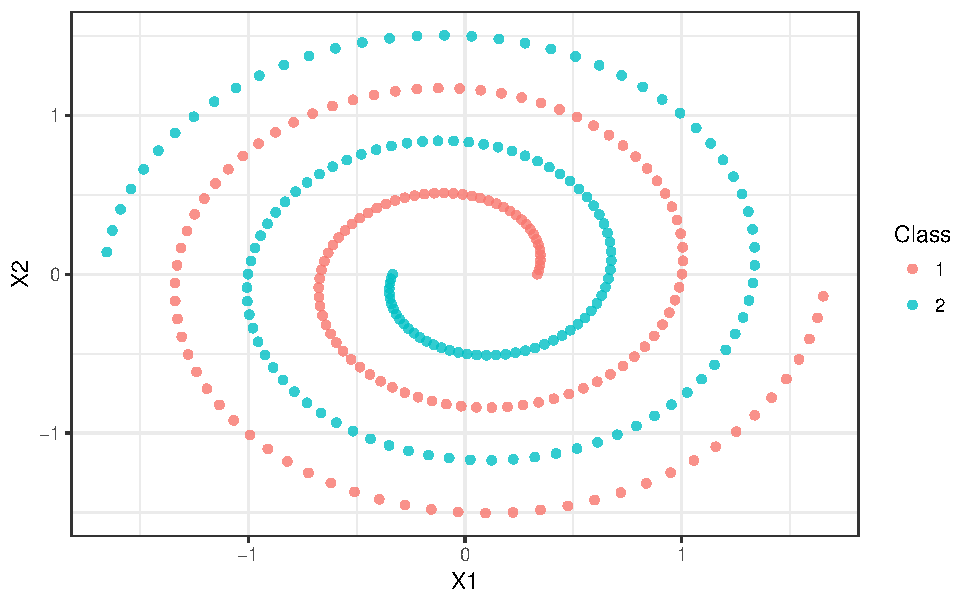
\includegraphics[width=0.7\textwidth]{figure/05-example_data}
  \caption{A scatter plot of simulated spiral data set.}
  \vspace{-0.5em}
  \label{fig:exampleiprobit}
\end{figure}

The three methods pretty much concur on the estimation of the intercept, but not on the RKHS scale parameter.
As a result, the log-density value calculated at the parameter estimates is also different in all three methods.
Notice the high posterior standard deviation for the scale parameter in the HMC method.
The posterior density for $\lambda$ was very positively skewed, and this contributed to the large posterior mean.

\begin{table}[hbt]
\centering
\caption[Table comparing various estimation methods for I-probit model]{Table comparing the estimated parameter values, (marginal) log-likelihood values, and also time taken (in seconds) for the three estimation methods.}
\label{tab:compreiprobit}
\begin{tabular}{@{}lrrr@{}}
\toprule
& Laplace approximation 
& Variational EM 
& Hamiltonian MC          \\ \midrule
Intercept ($\alpha$)      & -0.02 (0.03)           & 0.00 (0.06)    & 0.00 (0.58)  \\
Scale ($\lambda$)      & 0.85 (0.01)         & 5.67 (0.23)  & 29.3 (5.21)     \\[0.5em]
Log-density    & -171.8              & -43.2       & -8.5                  \\
Error rate (\%) & 44.7               & 0.00        & 0.00                   \\
Brier score & 0.20               & 0.02        & 0.01                   \\[0.5em]
Iterations     & 20                  & 56          & 2000                    \\
Time taken (s) & >3600                & 5.32         & >1800                     \\ \bottomrule
\end{tabular}
\end{table}


\begin{figure}[p]
  \centering
  \vspace{1em}
  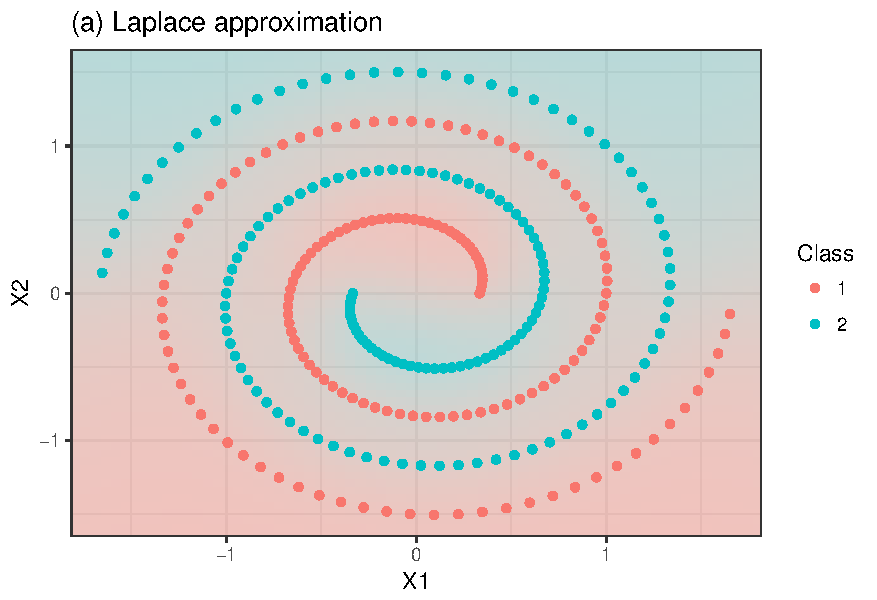
\includegraphics[width=0.49\textwidth]{figure/05-fit_lap}
  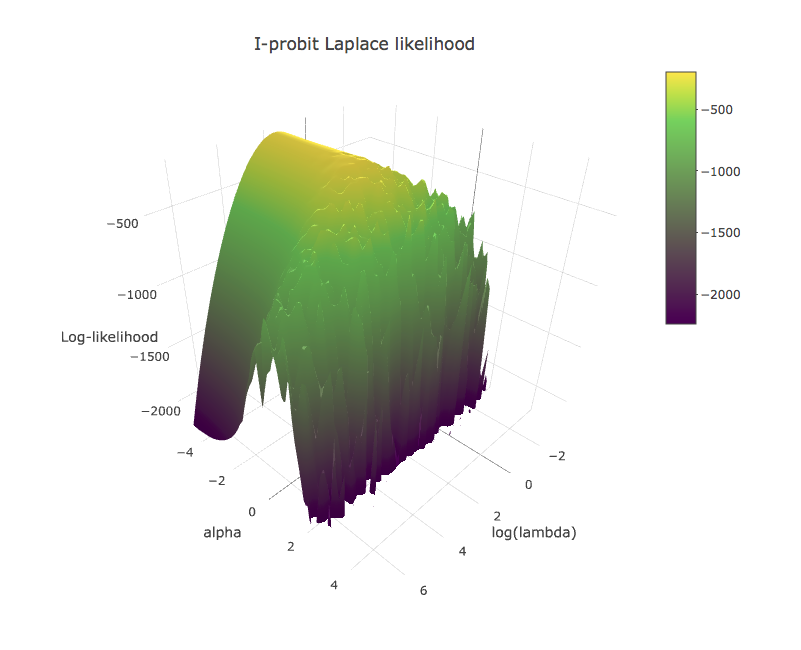
\includegraphics[width=0.49\textwidth]{figure/05-lik_lap}
  \vspace{1em}
  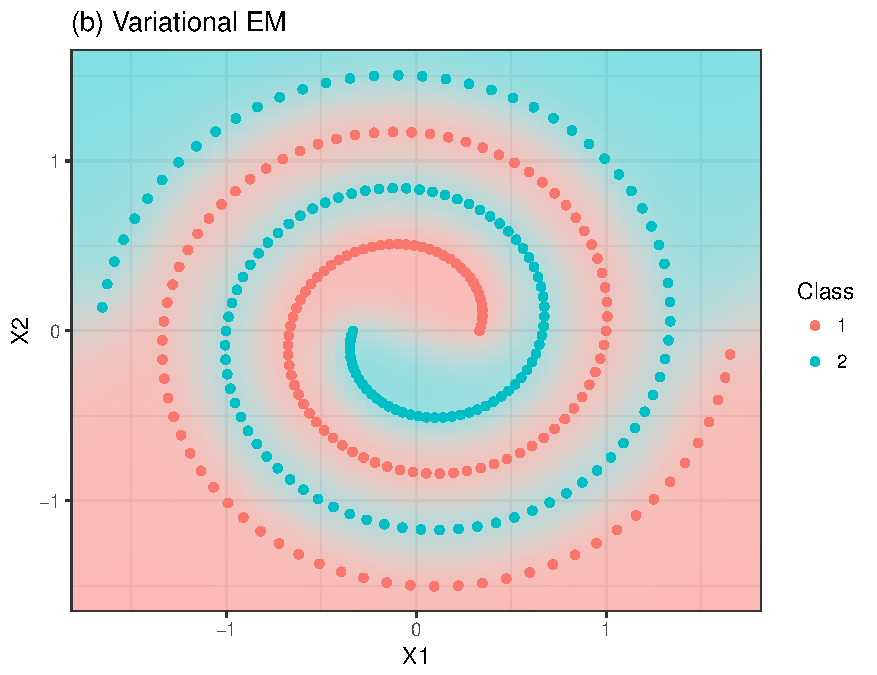
\includegraphics[width=0.49\textwidth]{figure/05-fit_vi}
  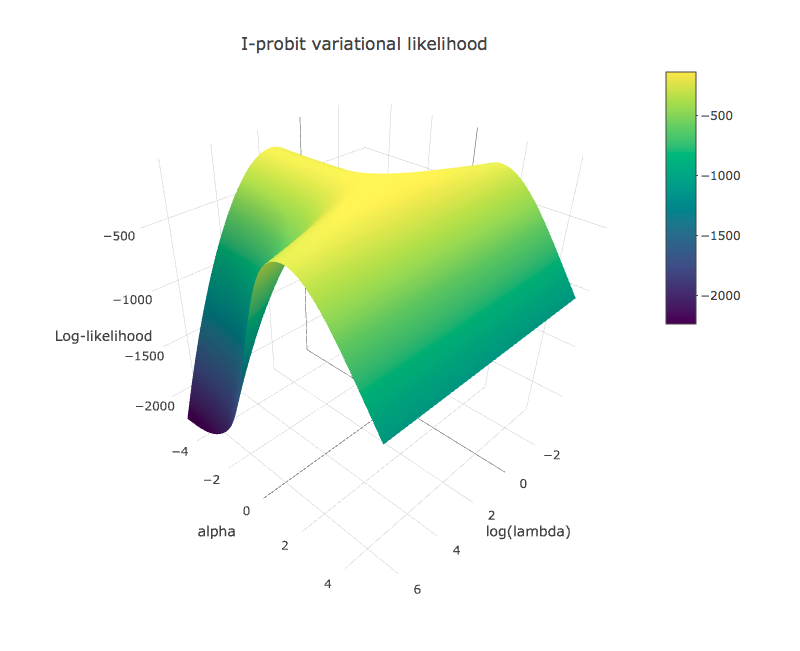
\includegraphics[width=0.49\textwidth]{figure/05-lik_vi}
  \vspace{1em}
  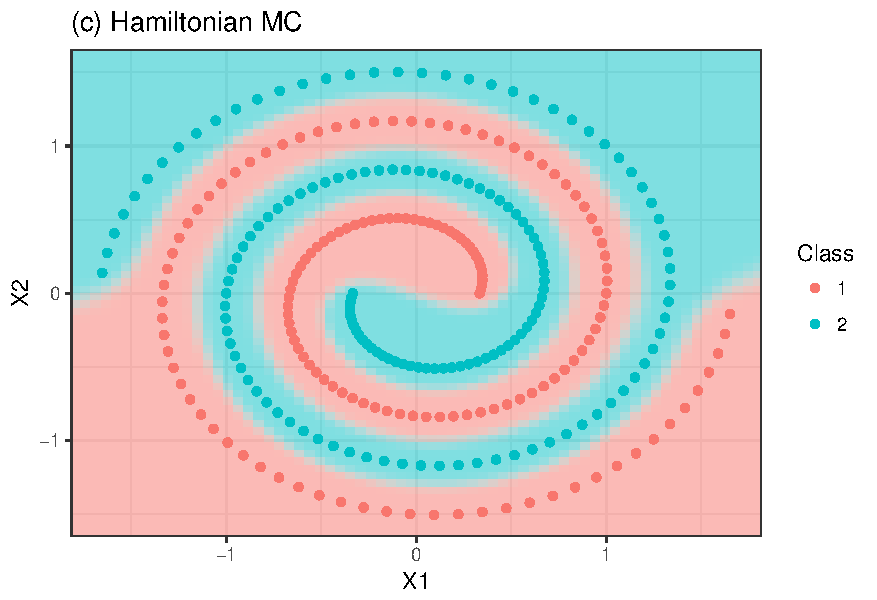
\includegraphics[width=0.49\textwidth]{figure/05-fit_hmc}
  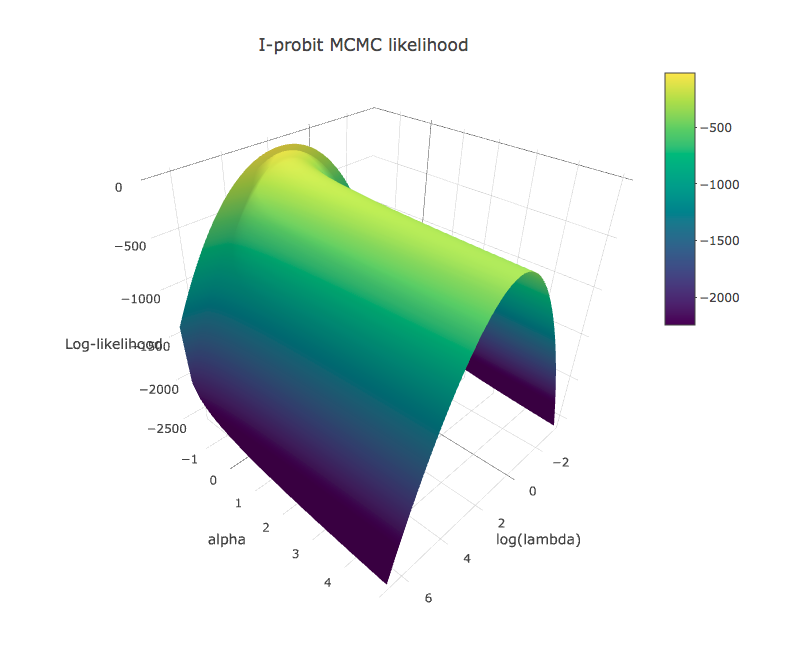
\includegraphics[width=0.49\textwidth]{figure/05-lik_hmc}
  \caption[Predicted I-probit probabilities and log-density plots]{Plots showing predicted probabilities (shaded region) for belonging to class `1' or `2' indicated by colour and intensity, and log-likelihood/ELBO surface plots for (a) Laplace's method, (b) variational EM, and (c) HMC. For the likelihood plot relating to Hamiltonian Monte Carlo, parameters are treated as fixed, and the mean log-density of the I-probit model recorded.}
  \label{fig:exampleiprobitfit}
\end{figure}
\index{Brier score}

\index{Laplace's method}
A plot of the log-likelihood (or ELBO) surface for three methods in \cref{fig:exampleiprobitfit} reveals some insight.
The variational likelihood has two ridges, with the maxima occurring around the intersection of these two ridges.
The Laplace likelihood seems to indicate a similar shape---in both the Laplace and variational method, the posterior distribution of $\bw$ is approximated by a Gaussian distribution, with different means and variances.
However, parts of the Laplace likelihood are poorly approximated resulting in a loss of fidelity around the supposed maxima, which might have contributed to the set of values that were estimated.
Laplace's method is known to yield poor approximations to probit model likelihoods \citep{kuss2005assessing}.
On the other hand, the log-likelihood calculated using an HMC sampler (treating parameters as fixed values) yields a slightly different graph: the log-likelihood increases as values of $\alpha$ become larger, resulting in the upwards inflection of the log-likelihood surface (as opposed to a downward inflection seen in the variational and Laplace likelihood).

In terms of predictive abilities, both the variational and  HMC methods, even though the posteriors are differently estimated, have good predictive performance as indicated by their error rates and Brier scores\footnote{\index{Brier score}The Brier score is defined as $\frac{1}{n}\sum_{i=1}^n\sum_{j=1}^m (y_{ij} - \hat p_{ij})$ with $y_{ij}=1$ if $y_i = j$ and zero otherwise, and $\hat p_{ij}$ is the fitted probability $\hat\Prob(y_i = j)$. It gives a better sense of training/test error, compared to simple misclassification rates, by accounting for the forecasted probabilities of the events happening. The Brier score is a proper scoring rule, i.e. it is uniquely minimised by the true probabilities.}.
\cref{fig:exampleiprobitfit} shows that HMC is more confident of new data predictions compared to variational inference, as indicated by the intensity of the shaded regions (HMC is shaded stronger than variational EM).
Laplace's method gave poor predictive performance.

Finally, on the computational side, variational inference was by far the fastest method to fit the model.
Sampling using HMC was very slow, because the parameter space is in effect $O(n + 2)$ (parameters are $\{w_1,\dots,w_n,\alpha,\lambda\}$ under the model with likelihood \cref{eq:intractablelikelihood2}, i.e. without the data augmentation scheme).
As for Laplace, each Newton step involves obtaining posterior modes of the $w_i$'s, and this contributed to the slowness of this method.
The reality is that variational inference takes seconds to complete what either the Laplace or full MCMC methods would take minutes or even hours to.
The predictive performance, while not as good as HMC, is certainly an acceptable compromise in favour of speed.
\vspace{-1em}
